% \section{Convolutional Neural Networks (CNN)}
% Convolutional Neural Networks (CNNs) are a class of deep learning models that have become the foundation for many computer vision tasks, such as image classification, object detection, and segmentation. CNNs are specifically designed to process grid-like data, such as images, by leveraging the hierarchical pattern in images to automatically learn spatial hierarchies of features. The architecture of a CNN is composed of multiple layers, including convolutional layers, pooling layers, and fully connected layers, as shown in figure \ref{fig:cnn}. CNNs are particularly efficient in processing images due to their ability to capture local dependencies while maintaining translation invariance.

% The core component of a CNN is the Convolutional Layer, where a filter (or kernel) is convolved with the input image to extract features such as edges, textures, and patterns. The filter slides over the image with a specified stride, and the result of this convolution is passed through a non-linear activation function, typically the Rectified Linear Unit (ReLU) \cite{goodfellow2016deep}. This operation allows the network to detect low-level features in the early layers and more complex patterns in deeper layers.

% Following the convolutional layer, a Pooling Layer is often applied, which reduces the spatial dimensions of the feature maps. The most common pooling operation is max-pooling, where the maximum value from a region is selected, reducing the size of the feature map while preserving important information. This helps to make the model more invariant to small translations of the image.

% Finally, the fully connected layers at the end of the network help in classification by using the features extracted from the convolutional layers and pooling layers to make predictions. The last fully connected layer typically uses a softmax activation function for multi-class classification tasks.

% In summary, CNNs are a powerful class of models in deep learning that are particularly suited for image-related tasks due to their ability to learn hierarchical feature representations efficiently.

% \begin{figure}[hbt]
%     \centering
%     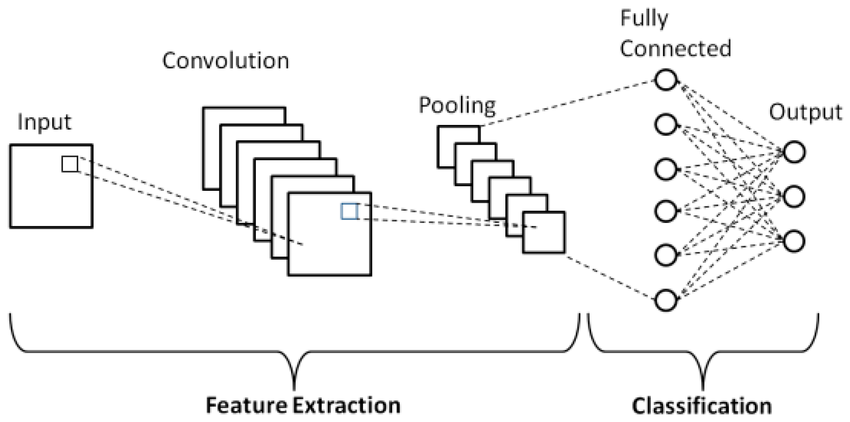
\includegraphics[width=1\textwidth]{theoretical-background/image/cnn.png}
%     \caption{Schematic diagram of a basic Convolutional Neural Network (CNN) architecture.}
%     \label{fig:cnn}
% \end{figure}


% \textbf{Convolution Operation}: The convolution operation in CNNs is defined as follows. Given an input image $I$ and a filter $K$, the convolution operation produces an output feature map $O$. The output is calculated by taking the dot product between the filter and the image at each location as the filter slides over the image.

% \begin{align}
% O(i,j) = (I * K)(i,j) = \sum_m \sum_n I(i+m, j+n) \cdot K(m,n)
% \end{align}

% \textbf{Max Pooling}: Max-pooling is used to reduce the spatial dimensions of the feature map by selecting the maximum value in a specified window, often $2 \times 2$. This operation helps to decrease the computational load while preserving the most important features.

% \begin{align}
% \text{MaxPool}(I) = \max(I)
% \end{align}

% \textbf{Fully Connected Layer}: After the convolution and pooling operations, the flattened output is passed through a fully connected layer. This layer is a standard neural network layer where each neuron is connected to every neuron in the previous layer. The output of this layer is typically passed through an activation function like softmax for classification tasks.
% \begin{align}
% FC(x) = W \cdot x + b
% \end{align}